%\documentclass[mathserif]{beamer}
\documentclass[handout]{beamer}
%\usetheme{Goettingen}
\usetheme{Warsaw}
%\usetheme{Singapore}
%\usetheme{Frankfurt}
%\usetheme{Copenhagen}
%\usetheme{Szeged}
%\usetheme{Montpellier}
%\usetheme{CambridgeUS}
%\usecolortheme{}
%\setbeamercovered{transparent}
\usepackage[english, activeacute]{babel}
\usepackage[utf8]{inputenc}
\usepackage{amsmath, amssymb}
\usepackage{dsfont}
\usepackage{graphics}
\usepackage{cases}
\usepackage{graphicx}
\usepackage{pgf}
\usepackage{epsfig}
\usepackage{amssymb}
\usepackage{multirow}	
\usepackage{amstext}
\usepackage[ruled,vlined,lined]{algorithm2e}
\usepackage{amsmath}
\usepackage{epic}
\usepackage{epsfig}
\usepackage{fontenc}
\usepackage{framed,color}
\usepackage{palatino, url, multicol}
\usepackage{listings}
%\algsetup{indent=2em}


\vspace{-0.5cm}
\title{Bayesian Linear Regression}
\vspace{-0.5cm}
\author[Felipe Bravo Márquez]{\footnotesize
%\author{\footnotesize  
 \textcolor[rgb]{0.00,0.00,1.00}{Felipe José Bravo Márquez}} 
\date{ \today }




\begin{document}
\begin{frame}
\titlepage


\end{frame}


%%%%%%%%%%%%%%%%%%%%%%%%%%%


\begin{frame}{Bayesian Linear Regression}
\scriptsize{
\begin{itemize}
\item In this class, which  is mostly based on chapter 4 of \cite{mcelreath2020statistical}, we are going to revisit the linear regression model from a Bayesian point of view.


\item The idea is the same: to model the relationship of a numerical dependent variable $\mathbf{y}$ with $m$ independent variables  $\mathbf{x}_1, \mathbf{x}_2, \dots, \mathbf{x}_m$ from a dataset $d$.

\item The response variable $\mathbf{y}$ is again modeled with a Gaussian distribution: $y_i \sim N(\mu_i,\sigma^2)$.


\item We also maintain the assumption that each attribute has a linear relationship to the mean of the outcome.

\begin{displaymath}
\mu_i = \beta_0 + \beta_1 x_i + \dots \beta_m x_m
\end{displaymath}

\item However, we are not going to use least squares or maximum likelihood to obtain point estimates of the parameters.

\item Instead, we are going to estimate the joint posterior distribution of all the parameters of the model:

\begin{displaymath}
f(\theta|d)= f(\beta_0,\beta_1,\dots,\beta_m,\sigma|d)
\end{displaymath}







 
\end{itemize}



} 

\end{frame}



\begin{frame}{Bayesian Linear Models}
\scriptsize{
\begin{itemize}


\item The Bayesian linear regression is  more flexible than least squares as it allows incorporating prior information.

\item It also allows to interpret the uncertainty of the model in a much richer way.

\item Notice that the the parameters of the model are $\beta_0,\beta_1,\dots,\beta_m$ and $\sigma$ but not $\mu_i$.

\item This is because $\mu_i$ it is determined deterministically from the linear model's coefficients.

\item In order to build our posterior we need to define a likelihood function:

\begin{displaymath}
 f(d|\beta_0,\beta_1,\cdots,\beta_m,\sigma) =\prod_{i=1}^n f(d_i|\beta_0,\beta_1,\cdots,\beta_m,\sigma) 
\end{displaymath}


\item Where $d_i$ corresponds to each data point in the dataset $d$ containing $n$ values for $y$ and $x_1,\dots,x_m$ (IID assumption).

\item The likelihood of each point is modeled with a Gaussian distribution:

\begin{displaymath}
 f(d_i|\beta_0,\beta_1,\cdots,\beta_m,\sigma)= N(\mu_i, \sigma^2)
\end{displaymath}



 
\end{itemize}



} 

\end{frame}



\begin{frame}{Bayesian Linear Models}
\scriptsize{
\begin{itemize}


\item Now we need a joint prior density:

\begin{displaymath}
f(\theta)= f(\beta_0,\beta_1,\dots,\beta_m,\sigma)
\end{displaymath}


\item And the posterior gets specified as follows:

\begin{displaymath}
f(\theta|d)= \frac{ \prod_{i=1}^n f(d_i|\beta_0,\beta_1,\cdots,\beta_m,\sigma)*f(\beta_0,\beta_1,\dots,\beta_m,\sigma)}{f(d)}
\end{displaymath}


\item The evidence is expressed by a multiple integral:

\begin{displaymath}
 f(d) = \int \int \dots \int \prod_{i=1}^n f(d_i|\beta_0,\beta_1,\cdots,\beta_m,\sigma)* f(\beta_0,\beta_1,\dots,\beta_m,\sigma) d\beta_0 d\beta_1 \cdots d\beta_md\sigma
\end{displaymath}



\item In most cases, the priors are specified independently for each parameter, which is equivalent to assuming:


\begin{displaymath}
f(\beta_0,\beta_1,\cdots,\beta_m,\sigma)=f(\beta_0)*f(\beta_1)*\dots*f(\beta_m)*f(\sigma). 
\end{displaymath}






 
\end{itemize}



} 

\end{frame}



\begin{frame}{A model of height revisited}
\scriptsize{
\begin{itemize}
 \item   To understand this more concretely, we will rebuild the linear model relating the height and weight of the !Kung San people using a Bayesian approach.
 
 \item We will refer to each person's height and weight as $y_i$ and $x_i$ respectively.
 
 \item Our probabilistic model specifying all components of a Bayesian model is defined as follows:
 
 \vspace{0.3cm}
 \begin{table}
 \centering
 \begin{tabular}{lr}  
$y_i \sim N(\mu_i,\sigma)$ & [likelihood] \\
$\mu_i = \beta_0 + \beta_1 x_i$ & [linear model] \\
$\beta_0 \sim N(150,50)$ & [$\beta_0$ prior] \\
$\beta_1 \sim N(0,1)$ & [$\beta_1$ prior] \\
$\sigma \sim $ Uniform$(0,50)$ & [$\sigma$ prior] \\
\end{tabular}
\end{table}

 \vspace{0.3cm}

 \item   Parameters $\beta_0$ and $\beta_1$ are the intercept and the slope of our linear model.
 
 \item The parameter $\sigma$ is the standard deviation of all the heights.
 
 \item Note that we are setting the same $\sigma$ for all observations, which is equivalent to the Homoscedasticity property of the standard linear regression. 
 


 
\end{itemize}
 

 
}
\end{frame}


\begin{frame}{A model of height revisited}
\scriptsize{
\begin{itemize}
 
  \item  Our priors were set independently for each parameter which implies that the joint prior density $f(\beta_0,\beta_1,\sigma)$ can be expressed as $f(\beta_0)*f(\beta_1)*f(\sigma)$.
 
 \item It should be kept in mind that the choice of priors is subjective and should be evaluated accordingly.
 
 \item Let's try to justify our choice a bit:
 
 \begin{enumerate}
 \scriptsize{
  \item The Gaussian prior for $\beta_0$ (intercept), centered on 150cm with a standard variation of 50, covers a huge range of plausible mean heights for human populations while giving very little chance for negative heights. \vspace{0.2cm}
  \item The Gaussian prior for $\beta_1$ (slope), centered on 0 with a standard variation of 1, acts as a \textbf{regularizer} to prevent the model from \textbf{overfitting} the data by assigning extreme values to $\beta_1$.\footnote{Regularization and overfitting will be discussed later in the course.}  \vspace{0.2cm} 
    \item The uniform prior for the standard deviation $\sigma$ between 0 and 50 prohibits obtaining negative standard deviations. The upper bound (50 cm) would imply that 95\% of individual heights lie within 100cm of the average height. That's a very large range.  \vspace{0.2cm}
}
 \end{enumerate}

  

 
\end{itemize}
 

 
}
\end{frame}


\begin{frame}[fragile]{Fitting the Model}
\scriptsize{
\begin{itemize}
 
  \item Now we need to fit the model to the data to build the posterior distribution.
  
  \item Grid approximation is not a valid option, as setting up a grid for 3 parameters would be too computationally expensive.
  
  \item We will use Laplace approximation instead.
  
  \item In this approach we obtain the MAP estimates for each parameter using a hill-climbing \textbf{optimization} method.
  
  \item Then we fit a \textbf{multivariate Gaussian distribution} centered on these values.
  
  
  \item This distribution is the multidimensional extension to the standard Gaussian.
  

 
\end{itemize}
 

 
}
\end{frame}

\begin{frame}[fragile]{The multivariate Gaussian distribution}
\scriptsize{
\begin{itemize}
 
  \item The multivariate Gaussian distribution in $m$-dimensions is defined by the following density function (PDF):
  
  \begin{displaymath}
   f_x = \frac{1}{(2\pi)^{m/2}|\Sigma|^{1/2}}\exp \left( -\frac{1}{2}(\vec{x}-\vec{\mu})^T  \Sigma^{-1}(\vec{x}-\mu)\right)
  \end{displaymath}

  
\item This density function allows working with a $m$-dimensional vector of random variables $\vec{X}$.


\item The first parameter of this distributions is a mean vector $\vec{\mu} \in \mathcal{R}^m$ with the mean value of each dimension.

\item The second parameter is a covariance matrix $\Sigma \in R^{m\times m}$.

\item This matrix contains the variance of each variable in the diagonal and the covariance of variables $X_i$ and $X_j$ in the other cells $\Sigma_{i,j}$:

\begin{displaymath}
 Cov(X) = \Sigma
\end{displaymath}

\item The matrix $\Sigma$ is symmetric and positive semi-definite.
  
\item The multivariate Gaussian $N(\vec{\mu},\Sigma)$ is a very convenient distribution for modeling multidimensional random variables.
  
  
 
\end{itemize}
 

 
}
\end{frame}



\begin{frame}[fragile]{The multivariate Gaussian distribution}
\scriptsize{
\begin{itemize}
 
  \item Here are some examples taken from \cite{ng2008generative} of what the density of a multivariate Gaussian distribution looks like:
  
  \begin{figure}[h!]
	\centering
	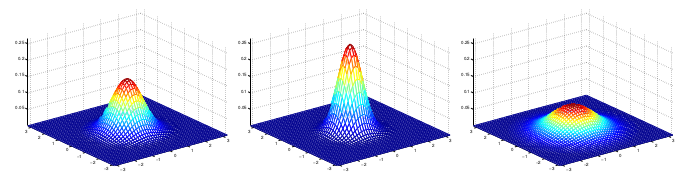
\includegraphics[scale=0.4]{pics/mgaussian1.png}
\end{figure}


\item The left-most figure shows a Gaussian with mean zero (that is, the 2x1 zero-vector) and covariance matrix $\Sigma = I$ (the $2\times2$ identity matrix). 
\item A Gaussian with zero mean and identity covariance is also called the standard normal distribution.

\item The middle figure shows the density of a Gaussian with zero mean and $\Sigma = 0.6I$.

\item The rightmost figure shows one with $\Sigma = 2I$.

\item We see that as $\Sigma$ becomes larger, the Gaussian becomes more ``spread-out'', and as it becomes smaller, the distribution becomes more ``compressed''.
 
\end{itemize}
 

 
}
\end{frame}





\begin{frame}[fragile]{The multivariate Gaussian distribution}
\scriptsize{


  
  \begin{figure}[h!]
	\centering
	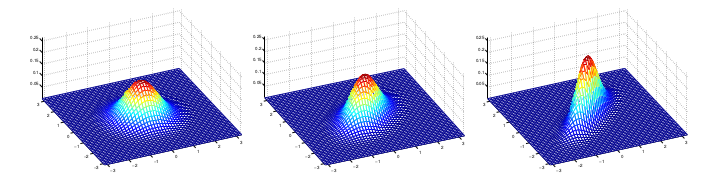
\includegraphics[scale=0.4]{pics/mgaussian2.png}
\end{figure}
 
\begin{itemize}
 

 \item The figures above show Gaussians with mean 0, and with covariance matrices respectively
 
   \begin{figure}[h!]
	\centering
	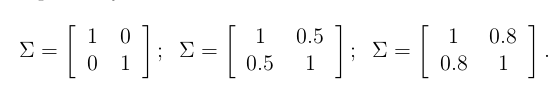
\includegraphics[scale=0.35]{pics/mgaussian4.png}
\end{figure}

\item The leftmost figure shows the familiar standard normal distribution, and we see that as we increase the off-diagonal entry in $\Sigma$, the density becomes more ``compressed'' towards the $45\cdot$ line (given by $x_1 = x_2$).
 
\end{itemize}
 

 
}
\end{frame}





\begin{frame}[fragile]{The multivariate Gaussian distribution}
\scriptsize{
\begin{itemize}
 
  \item   As our last set of examples, fixing $\Sigma = I$, by varying $\vec{\mu}$ we can also move the mean of the density around.
  
  \begin{figure}[h!]
	\centering
	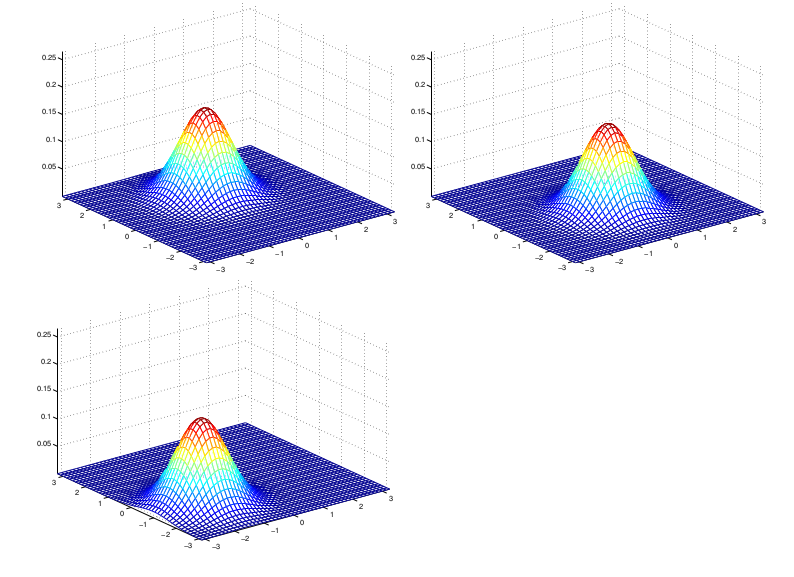
\includegraphics[scale=0.25]{pics/mgaussian3.png}
\end{figure}
 

 \item The figures above were generated using $\Sigma = I$, and respectively
 
   \begin{figure}[h!]
	\centering
	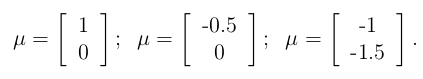
\includegraphics[scale=0.3]{pics/mgaussian5.png}
\end{figure}
 
\end{itemize}
 

 
}
\end{frame}


\begin{frame}{Laplace approximation}
\scriptsize{

\begin{itemize}
\item In Laplace approximation we assume that the joint posterior follows a multivariate Gaussian distribution $f(\theta_1,\dots,\theta_m) = N(\vec{\mu},\Sigma)$.

\item  According to \cite{gelman2013bayesian}, this approximation is convenient for unimodal and roughly symmetric posterior distributions.

\item There are also a theoretical asymptotic argument in favor of this approximation: ``if the dataset is large enough, a posterior distribution can be approximated by a Gaussian'' \cite{gelman2013bayesian}.

\item The values of $\vec{\mu}$ are obtained from the posterior mode of each parameter (MAP):
\begin{displaymath}
 \vec{\mu} = \vec{\theta}_{MAP}
\end{displaymath}

\item Which are obtained using numeric optimization techniques.


\end{itemize}


} 
\end{frame}



\begin{frame}{Laplace approximation}
\scriptsize{

\begin{itemize}

\item The values of $\Sigma$ are obtained from the curvature near these values, which are obtained from the second derivatives of the posterior:

\begin{displaymath}
 \Sigma = [I({\theta}_{MAP})]^{-1}
\end{displaymath}

where  \begin{displaymath}
        I(\theta) = - \frac{d^2}{d\theta^2} \log f(\theta|d)
       \end{displaymath}



\item Notice that both  $\vec{\mu}$ and $\Sigma$ can be calculated from the unnormalized posterior 
$f(d|\theta)*f(\theta)$

\item We don't need to calculate the evidence $f(d)$ to perform Laplace approximation \cite{laplaceApp}.

\end{itemize}


} 
\end{frame}


\begin{frame}[fragile]{Fitting the Model}
\scriptsize{
\begin{itemize}
 
  \item Laplace approximation is implemented in the \textbf{quap} function from the \textbf{rethinking} package.
  
  \item The model for height defined above can be implemented as follows:
  
  \begin{verbatim}
library(rethinking)
data(Howell1)
d <- Howell1
d2 <- d[ d$age >= 18 , ]

b.reg1 <- quap(
  alist(
    height ~ dnorm( mu, sigma ),
    mu <- b0 + b1*weight,
    b0 ~ dnorm( 150 , 50 ) ,
    b1 ~ dnorm( 0 , 1) ,
    sigma ~ dunif( 0 , 50 )
  ) , data=d2 )
  \end{verbatim}

  

 
\end{itemize}
 

 
}
\end{frame}

\begin{frame}[fragile]{Fitting the Model}
\scriptsize{
\begin{itemize}
 
  \item We can summarize this posterior with the command \textbf{precis}:
  
  \begin{verbatim}
> precis( b.reg1, prob=0.95 )
        mean   sd   2.5%  97.5%
b0    113.99 1.90 110.26 117.71
b1      0.90 0.04   0.82   0.98
sigma   5.07 0.19   4.70   5.45
  \end{verbatim}

\item These numbers provide Gaussian approximations for each parameter's \textbf{marginal} posterior distribution.

\item The marginal of multivariate distribution is the univariate distribution of a single parameter $\theta_i$ after integrating (averaging) over all the other parameters  $\theta_j \ \forall j \neq i$:

\begin{displaymath}
f(\theta_i |d) = \int \dots \int f(\theta_1,\dots,\theta_m|d)d\theta_1,\dots,d\theta_{i-1},d\theta_{i+1},\dots,d\theta_{m} 
\end{displaymath}

 
\end{itemize}
 

 
}
\end{frame}


\begin{frame}[fragile]{Fitting the Model}
\scriptsize{
\begin{itemize}
 
  \item In a multivariate Gaussian $N(\vec{\mu},\Sigma)$, the marginal distribution of $\theta_i$ is a univariate Gaussian $N(\vec{\mu}_i,\Sigma_{ii})$. 

  \item So, the marginal distribution of $\beta_1$ is a Gaussian distribution with $\mu=0.9$ and $\sigma=1.9$. 
  
  \item The last two columns of the summary table show the lower and upper limits of a 95\% equal-tailed credible interval for each parameter.
  
  \item For the case of $\beta_1$, 95\% of the posterior probability lies between 0.82 and 0.98. 
  
  \item That suggests that $\beta_1$ values close to zero or greatly above one are highly incompatible with these data and this model.
 
\end{itemize}
 

 
}
\end{frame}


\begin{frame}[fragile]{Fitting the Model}
\scriptsize{
\begin{itemize}

\item Let's compare the mean and standard deviation of $\beta_0$ and $\beta_1$ with what we obtained using least squares in previous lecture:

\begin{verbatim}
> summary(reg1)
...

Coefficients:
             Estimate Std. Error t value Pr(>|t|)    
(Intercept) 113.87939    1.91107   59.59   <2e-16 ***
weight        0.90503    0.04205   21.52   <2e-16 ***
---
Signif. codes:  0 ‘***’ 0.001 ‘**’ 0.01 ‘*’ 0.05 ‘.’ 0.1 ‘ ’ 1

Residual standard error: 5.086 on 350 degrees of freedom
....
\end{verbatim}


\item These values are almost the same!

\item Recall that maximum likelihood or least squares estimators are identical to MAP estimators with uniform priors.

\item This indicates that our priors did not have a significant impact in the resulting posterior.



 
\end{itemize}
 

 
}
\end{frame}

\begin{frame}[fragile]{Covariance Matrix}
\scriptsize{
\begin{itemize}

\item We can also get the covariance matrix $\Sigma$ of our multivariate Gaussian obtained with Laplace approximation:

\begin{verbatim}
> vcov( b.reg1 )
                b0            b1         sigma
b0     3.620141920 -7.884254e-02  1.765417e-03
b1    -0.078842537  1.752477e-03 -3.830179e-05
sigma  0.001765417 -3.830179e-05  3.654305e-02 
\end{verbatim}


\item The matrix tell us  how each parameter relates to every other parameter in the posterior distribution.

\item It is better to turn them into correlations for easier interpretation:

\begin{verbatim}
> cov2cor( vcov( b.reg1 ) )
                b0           b1        sigma
b0     1.000000000 -0.989855066  0.004853802
b1    -0.989855066  1.000000000 -0.004786196
sigma  0.004853802 -0.004786196  1.000000000
\end{verbatim}

\item Notice that $\beta_0$ and $\beta_1$ are almost perfectly negatively correlated.

\item This means that these two parameters carry the same information: as we change the slope of the line, the best intercept changes to match it.


\end{itemize}
 

 
}
\end{frame}


\begin{frame}[fragile]{Centering}
\scriptsize{
\begin{itemize}
\item In more complex models, strong correlations like this can make it difficult to fit the model to the data. 

\item A useful trick to avoid this problem is  centering: subtract the mean of a variable from each value. 

\begin{verbatim}
d2$weight.c <- d2$weight - mean(d2$weight)
b.reg2 <- quap(
  alist(
    height ~ dnorm( b0 + b1*weight.c, sigma ),
    b0 ~ dnorm( 150 , 50 ) ,
    b1 ~ dnorm( 0 , 1) ,
    sigma ~ dunif( 0 , 50 )
  ) , data=d2 )

> cov2cor( vcov( b.reg2 ) )
                 b0            b1         sigma
b0     1.000000e+00  6.901851e-08 -2.435168e-05
b1     6.901851e-08  1.000000e+00 -2.860675e-03
sigma -2.435168e-05 -2.860675e-03  1.000000e+00  
\end{verbatim}

\item The correlations among parameters are now all very close to zero.

\end{itemize}
 

 
}
\end{frame}


\begin{frame}[fragile]{Sampling from the Posterior}
\scriptsize{
\begin{itemize}
\item In the remainder of this class we will work with samples from our multi-dimensional posterior.
\item The rethinking package provides the \textbf{extract.samples} function to obtain them:
\begin{verbatim}
> post <- extract.samples( b.reg1, n= 1e4 )
> head(post)
        b0        b1    sigma
1 112.6949 0.9241772 5.379502
2 114.0312 0.9049003 5.213418
3 114.5932 0.8867978 5.057051
4 111.9088 0.9522044 5.021026
5 111.7631 0.9496914 4.886909
6 116.6987 0.8367835 5.256882
\end{verbatim}

\item Each sample is a different line relating height and weight.

\item Bear in mind that each line is sampled in proportion to the posterior probabilities, which represent our model's beliefs.




\end{itemize}
 

 
}
\end{frame}


\begin{frame}[fragile]{Sampling from the Posterior}
\scriptsize{
\begin{itemize}
\item We can see that the mean of each variable in the sample is almost identical to the corresponding MAP estimate:

\begin{verbatim}
> sapply(post,mean)
         b0          b1       sigma 
114.0026648   0.9023462   5.0693261  
\end{verbatim}



\item Since our posterior was approximated with Laplace approximation, we can obtain equivalent samples directly from a multi-variate Gaussian using the \textbf{mvrnorm} function:


\begin{verbatim}
> library(MASS)
> post2 <- mvrnorm( n=1e4,mu=coef(b.reg1), 
Sigma=vcov(b.reg1 ) )
> post2<-as.data.frame(post2)
> sapply(post2,mean)
         b0          b1       sigma 
113.9997660   0.9023735   5.0691332 
\end{verbatim}




\end{itemize}
 

 
}
\end{frame}



\begin{frame}[fragile]{Plotting posterior inference against the data}
\scriptsize{
\begin{itemize}
\item In truth, tables of estimates are usually insufficient for understanding the information contained in the posterior distribution.

\item It's almost always much more useful to plot the posterior inference against the data.

\item We’re going to start with a simple version of that task, superimposing just the MAP values over the height and weight data.

\begin{verbatim}
plot( height ~ weight , data=d2 , col=rangi2 )
b0_map <- mean(post$b0)
b1_map <- mean(post$b1)
curve( b0_map + b1_map*x, add=TRUE ) 
\end{verbatim}



\end{itemize}
 

 
}
\end{frame}



\begin{frame}{Plotting posterior inference against the data}

\begin{figure}[h!]
	\centering
	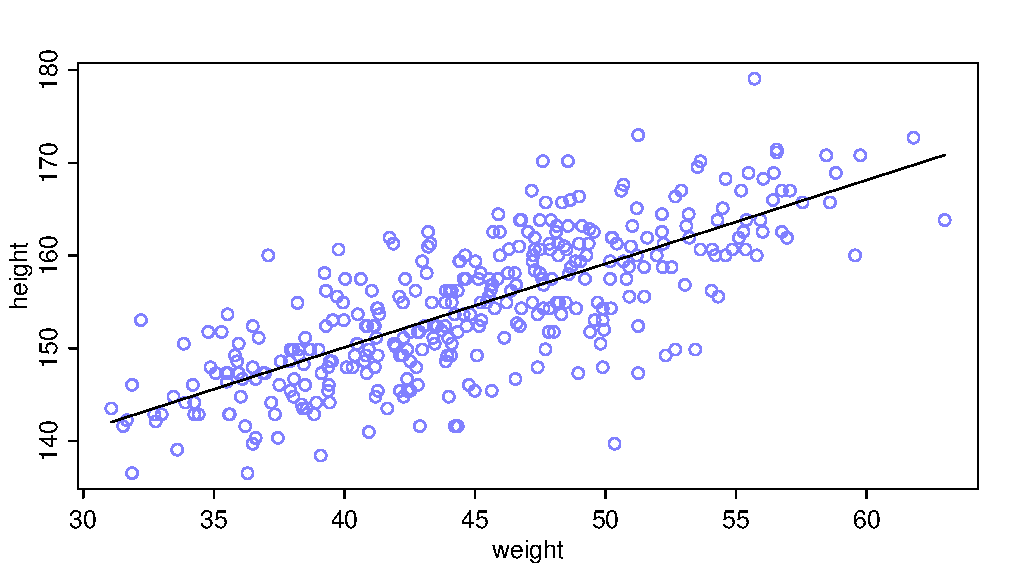
\includegraphics[scale=0.65]{pics/height_points.pdf}
\end{figure}

\end{frame}


\begin{frame}[fragile]{Plotting regression intervals}
\scriptsize{
\begin{itemize}
\item The previous plot doesn't incorporate the uncertainty embodied in the posterior.

\item This can be done by by plotting a credible interval around the MAP regression line.

\item To understand how it works, let's focus for the moment on a single weight value, say 50 kilograms. 

\item We can quickly make a list of 10,000 values of $\mu$ for an individual who weighs 50 kilograms, by using our samples from the posterior:

\begin{verbatim}
mu_at_50 <- post$b0 + post$b1 * 50 
\end{verbatim}

\item It might be helpful at this point to actually plot the density for this vector of means:

\begin{verbatim}
dens( mu_at_50 , col=rangi2 , lwd=2 , xlab="mu|weight=50" )
\end{verbatim}


\end{itemize}
 

 
}
\end{frame}

\begin{frame}{Plotting regression intervals}

\begin{figure}[h!]
	\centering
	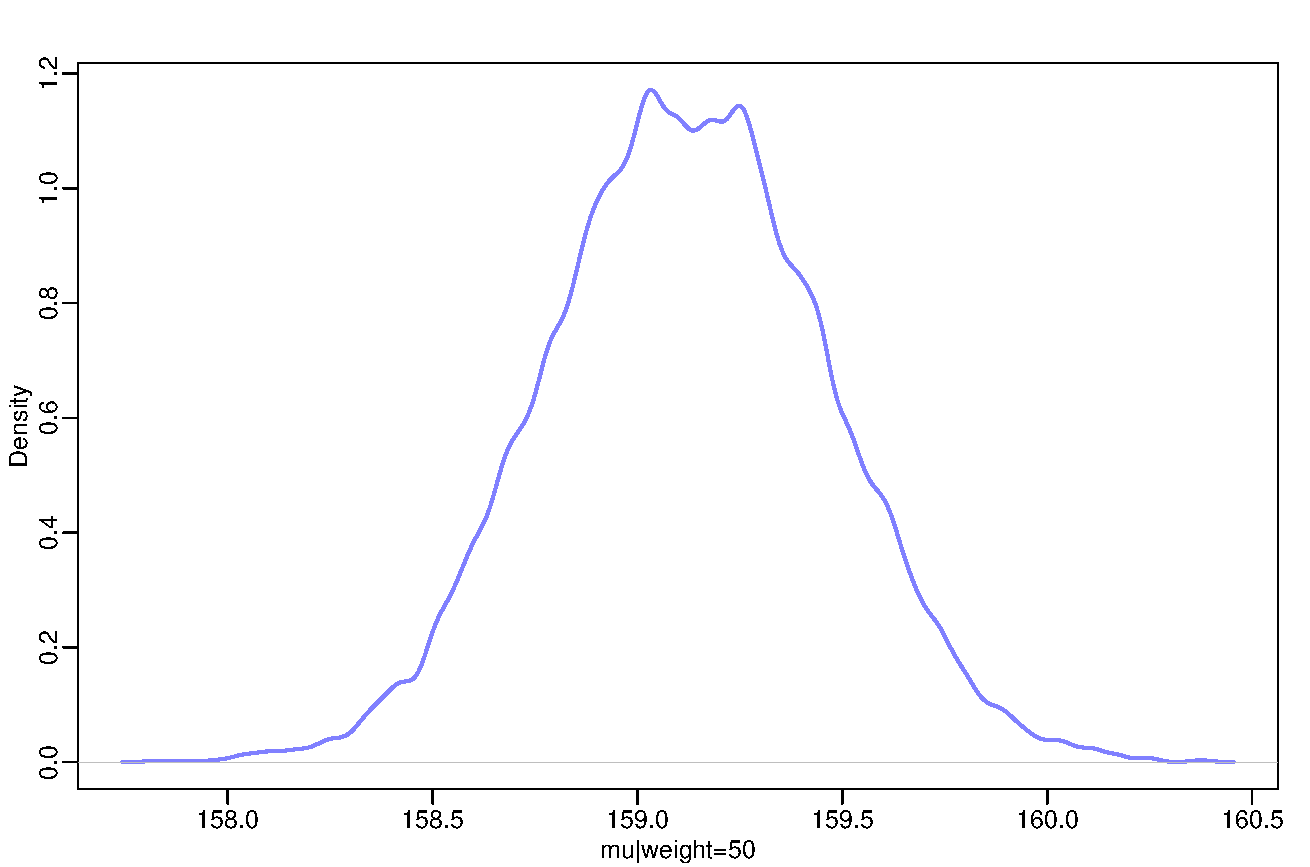
\includegraphics[scale=0.45]{pics/mu50.pdf}
\end{figure}

\end{frame}


\begin{frame}[fragile]{Plotting regression intervals}
\scriptsize{
\begin{itemize}
\item Since the components of $\mu$ have distributions ($\beta_0,\beta_1$), so too does $\mu$.

\item And since the distributions of $\beta_0$ and $\beta_1$ are Gaussian, so to is the distribution of $\mu$.

\item Adding Gaussian distributions always produces a Gaussian distribution.

\item Since the posterior for $\mu$ is a distribution, you can find intervals for it, just like for any posterior distribution. 

\item To find the 89\% highest posterior density interval of $\mu$ at 50 kg, we just use the HPDI command as usual:

\begin{verbatim}
> HPDI( mu_at_50 , prob=0.95 )
   |0.95    0.95| 
158.4883 159.8061  
\end{verbatim}

\item Now, we need to repeat the above calculation for every weight value on the horizontal axis, not just when it is 50 kg.

\end{itemize}
 

 
}
\end{frame}


\begin{frame}[fragile]{Plotting regression intervals}
\scriptsize{
\begin{itemize}


\item We first define a sequence of weights to compute predictions for:

\begin{verbatim}
weight.seq <- seq( from=25 , to=70 , by=1 ) 
\end{verbatim}

\item These values will be on the horizontal axis of our plot.

\item Now, for each of these weights we will compute a posterior distribution of the average height $\mu$ using samples from the posterior:

\begin{verbatim}
mu.link <- function(weight) post$b0 + post$b1*weight
\end{verbatim}

\item The function above will use the $1000$ different sampled regression lines to compute various values of $\mu$ for a given weight.

\item We can apply this function to all our 46 weights (from 25 to 70) and obtain a matrix of $1000 \times 46$:

\begin{verbatim}
> mu <- sapply( weight.seq , mu.link )
> dim(mu)
[1] 10000    46 
\end{verbatim}



\end{itemize}
 

 
}
\end{frame}


\begin{frame}[fragile]{Plotting regression intervals}
\scriptsize{
\begin{itemize}


\item Now, we can get a MAP value of $\mu$ for each weight, simply by by averaging the rows of the matrix:

\begin{verbatim}
> mu.mean <- apply( mu , 2 , mean )
> head(mu.mean)
[1] 136.5526 137.4555 138.3583 139.2612 140.1641 141.0669
\end{verbatim}

\item And we can get our 95\% HPDIs analogously:

\begin{verbatim}
mu.HPDI <- apply( mu , 2 , HPDI , prob=0.95 ) 
\end{verbatim}

\item The variable mu.HPDI contains 95\% lower and upper bounds for each weight value.

\item Now we can plot these intervals as shaded regions around the MAP estimates as follows:

\begin{verbatim}
plot( height ~ weight , data=d2 , col=col.alpha(rangi2,0.5) )
# plot the MAP line, aka the mean mu for each weight
lines( weight.seq , mu.mean )
# plot a shaded region for 95% HPPDI
shade( mu.HPDI , weight.seq ) 
\end{verbatim}


\end{itemize}
 

 
}
\end{frame}


\begin{frame}{Plotting regression intervals}

\begin{figure}[h!]
	\centering
	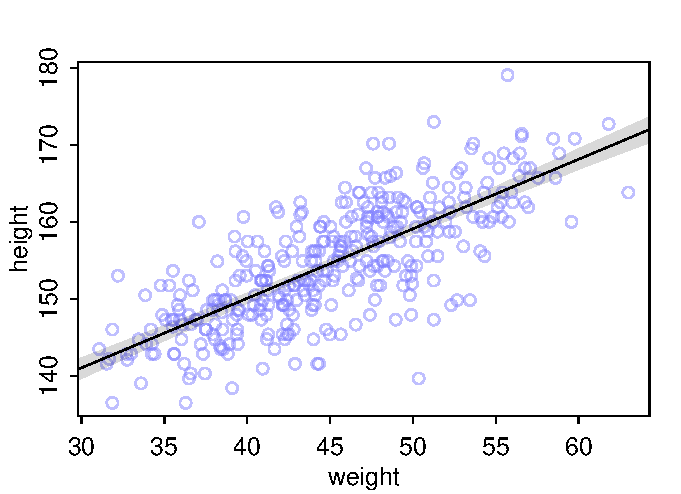
\includegraphics[scale=0.9]{pics/height_interval.pdf}
\end{figure}

\end{frame}

\begin{frame}[fragile]{Plotting regression intervals}
\scriptsize{
\begin{itemize}


\item In case of working with more complex linear models (i.e., multiple attributes, interactions) we can use the \textbf{link} function from the rethinking package:

\begin{verbatim}
mu <- link( b.reg1 , data=data.frame(weight=weight.seq),
n=1000 ) 
\end{verbatim}

\item This function will generate distributions of posterior values for $\mu$ using the formula declared in \textbf{quap} (e.g., $\mu= \beta_0 + \beta_1 * x$).

\item The default behavior of link is to use the original data.

\item So we have to pass it a list of new horizontal axis values we want to plot posterior predictions across.

\end{itemize}
 

 
}
\end{frame}


\begin{frame}[fragile]{Prediction Intervals}
\scriptsize{
\begin{itemize}


\item Now let’s walk through generating prediction intervals for simulated heights $\tilde{y}$ using the posterior predictive distribution.

\item What we did before was to use samples from the posterior to visualize the uncertainty in $\mu_i$ using the linear model of the mean: $\mu_i=\beta_0+\beta_1*x_i$. 

\item But actual predictions of heights $\tilde{y}$ depend also upon the stochastic definition of $y$ given in the likelihood function: $y_i\sim N(\mu_i,\sigma)$.

\item The Gaussian distribution of the likelihood tells us that the model expects observed heights $\tilde{y}$ to be distributed around $\mu$, not right on top of it. 

\item And the spread around $\mu$ is governed by $\sigma$. 

\item All of this suggests we need to incorporate $\sigma$ in the predictions somehow.

 


\end{itemize}
 

 
}
\end{frame}


\begin{frame}[fragile]{Prediction Intervals}
\scriptsize{
\begin{itemize}


\item The posterior predictive distribution introduced in previous class can exactly do that:

  \begin{displaymath}
 f(\tilde{y}|y)  =  \int_{\theta}f(\tilde{y}|\theta)f(\theta|y)d\theta 
 \end{displaymath}

\item For our height regression model it would take the following form: 

  \begin{displaymath}
 f(\tilde{y}|y)  = \int_{\beta_0} \int_{\beta_1} \int_{\sigma}f(\tilde{y}|\beta_0,\beta_1,\sigma)f(\beta_0,\beta_1,\sigma|y)d\beta_0 d\beta_1 d\sigma
 \end{displaymath}
 
where $f(\tilde{y}|\beta_0,\beta_1,\sigma)$ is the likelihood function $N(\beta_0+\beta_1*\tilde{x},\sigma^2)$ and $f(\beta_0,\beta_1,\sigma|y)$ is our posterior distribution.

\item Instead of working with these complex integrals we will simulate heights using samples from the posterior.

\end{itemize}
 

 
}
\end{frame}

\begin{frame}[fragile]{Prediction Intervals}
\scriptsize{
\begin{itemize}


\item Here's how we will do it. 

\item For any unique weight value, we sample from a Gaussian distribution with the correct mean $\mu$ for that weight, using the correct value of $\sigma$ sampled from the same posterior distribution.
\item We do this for every sample from the posterior and for every weight value of interest.

\item We end up with a collection of simulated heights that embody the uncertainty in the posterior as well as the uncertainty in the Gaussian likelihood.

\item We first need to implement a function that can generate a sample of heights for a given weight $w$.

\item The sampling should use the likelihood function $N(\beta_0+\beta_1*w,\sigma^2)$, using different values of  $\beta_0, \beta_1$ and $\sigma^2$ given by our posterior samples.

\begin{verbatim}
height.weight <- function(weight) 
  rnorm(
    n=nrow(post) ,
    mean=post$b0 + post$b1*weight ,
    sd=post$sigma )
\end{verbatim}



\end{itemize}
 

 
}
\end{frame}


\begin{frame}[fragile]{Prediction Intervals}
\scriptsize{
\begin{itemize}


\item Notice that we are passing  vectors of parameters $\vec{\mu}$ and $\vec{\sigma}$ to \textbf{rnorm} instead of scalars.

\item This will result in different samples generated with different parameter values:

\begin{verbatim}
> rnorm(4,mean=c(-100,100),sd=c(1,50))
[1]  -99.32946  126.17836 -100.62118  194.68311
\end{verbatim}

\item Now, we can apply this function to our sequence of weights and obtain a similar matrix  than before:

\begin{verbatim}
> sim.height <- sapply( weight.seq , height.weight)
> dim(sim.height)
[1] 10000    46 
\end{verbatim}

\item This matrix is much like the earlier one, but it contains simulated heights, not distributions of plausible average height, $\mu$.


\end{itemize}
 

 
}
\end{frame}


\begin{frame}[fragile]{Prediction Intervals}
\scriptsize{
\begin{itemize}


\item We can summarize these simulated heights in the same way we summarized the distributions of $\mu$, by using apply:

\begin{verbatim}
height.HPDI <- apply( sim.height , 2 , HPDI , prob=0.95 ) 
\end{verbatim}

\item Now height.HPDI contains the 95\% HPDIs of observable (according to the model) heights, across the values of weight in weight.seq.

\item Let's plot everything we've built up: (1) the MAP line, (2) the shaded region of 95\% plausible $\mu$, and (3) the boundaries of the simulated heights the model expects.

\begin{verbatim}
# plot raw data
plot( height ~ weight , d2 , col=col.alpha(rangi2,0.5) )
# draw MAP line
lines( weight.seq , mu.mean )
# draw HPDI region for line
shade( mu.HPDI , weight.seq )
# draw HPDI region for simulated heights
shade( height.HPDI , weight.seq ) 
\end{verbatim}




\end{itemize}
 

 
}
\end{frame}

\begin{frame}{Prediction Intervals}

\begin{figure}[h!]
	\centering
	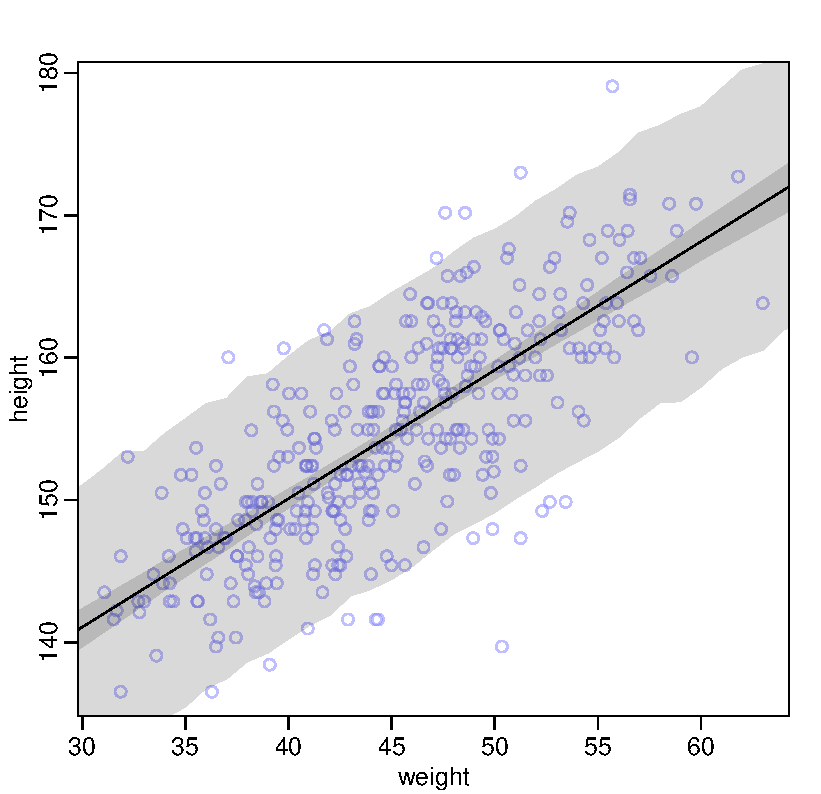
\includegraphics[scale=0.55]{pics/sim_height.pdf}
\end{figure}

\end{frame}


\begin{frame}[fragile]{Prediction Intervals}
\scriptsize{
\begin{itemize}


\item The two shaded regions of the figure show different 95\% plausible regions. 

\item The narrow shaded interval around the line is the
distribution of $\mu$. 
\item The wider shaded region represents the region within which the model expects to find 95\% of actual heights in the population, at each weight.

\item In the procedure above, we encountered both uncertainty in parameter values: $\beta_0,\beta_1,\sigma$, and uncertainty in a sampling process: $N(\mu_i,\sigma)$. 

\item These are distinct concepts, even though they are processed much the same way and end up blended together in the posterior predictive simulation.

\item Finally, the \textbf{sim} function of the rethinking package allows to easily generate samples of the posterior predictive distribution of any linear model declared with \textbf{quap}:

\begin{verbatim}
sim.height <- sim( b.reg1 , data=list(weight=weight.seq) )
 
\end{verbatim}



\end{itemize}
 

 
}
\end{frame}

\begin{frame}{Conclusions}
\scriptsize{

\begin{itemize}
\item In this class we have revisited the linear regression model using a Bayesian approach.

\item The posterior distribution can be interpreted as a distribution of possible lines.

\item We introduced Laplace approximation to fit these models to data.

\item We also introduced new procedures for visualizing posterior distributions and posterior predictions

\item In the next classes we will see more complex linear models, such as models with multiple attributes, binary attributes or interactions.

\item Notice that these models can also be built with \textbf{quap}.

\item However, a more sophisticated technique called Markov Chain Monte Carlo will allow us to sample from the posterior without making any assumptions about the posterior's shape.


\end{itemize}


} 
\end{frame}


%%%%%%%%%%%%%%%%%%%%%%%%%%%
\begin{frame}[allowframebreaks]\scriptsize
\frametitle{References}
\bibliography{bio}
\bibliographystyle{apalike}
%\bibliographystyle{flexbib}
\end{frame}  









%%%%%%%%%%%%%%%%%%%%%%%%%%%

\end{document}
